%-----------------------------------------------
% Dateiname: InstallTYPO3.tex
% Autor    : Stefano Kowalke <blueduck@gmx.net>
% Lizenz   : BSD
%-----------------------------------------------
\section{Installation von TYPO3 CMS}
\label{prototype:sec:installTYPO3}
\subsection{Verzeichnisse}
Zuerst wurde das Verzeichnis \pdf{thesis.dev/http} angelegt, welches als Wurzelverzeichnis der Installation über den Browser über die \textit{URL} erreichbar ist.

\begin{Verbatim}[samepage=true]
$ cd Sites/
$ mkdir -p thesis.dev/http/
$ cd thesis.dev/
\end{Verbatim}


Damit auf den Quellcode von TYPO3 CMS nicht über den Browser zugegriffen werden kann, wurde es per GIT nach \pdf{thesis.dev/typocms} heruntergeladen. Danach wurde nach \pdf{http} gewechselt und die notwendigen Symlinks und Verzeichnisse angelegt. Listing~\ref{lst:thesisDevFolders} zeigt die so erstellte Verzeichnisstruktur:

\begin{Verbatim}[samepage=true]
$ tree -L 2 --dirsfirst
.
├── http
│   ├── fileadmin
│   ├── typo3 -> typo3_src/typo3
│   ├── typo3_src -> ../typo3cms
│   ├── typo3conf
│   ├── uploads
│   └── index.php -> typo3_src/index.php
└── typo3cms
├── typo3
├── ChangeLog
├── GPL.txt
├── INSTALL.md
├── LICENSE.txt
├── NEWS.md
├── README.md
├── _.htaccess
├── composer.json
└── index.php
\end{Verbatim}

Danach wurde in der Hostdatei mittels \shinline{sudo sh -c "echo '127.0.0.1 thesis.dev' >> /etc/hosts"} ein A-Record der Domain \url{thesis.dev} angelegt und anschließend ein virtueller Host in der Apache2 Konfiguration erstellt, der auf das Verzeichnis \pdf{thesis.dev/http} zeigt.

\begin{shcode}
<VirtualHost *:80>¬
DocumentRoot "~/Sites/thesis.dev/http"¬
ServerName thesis.dev¬
ErrorLog "~/Sites/thesis.dev/logs/error_log"¬
CustomLog "~/Sites/thesis.dev/logs/access_log" common¬
</VirtualHost>
\end{shcode}

Im Anschluß daran wurde eine leere Datenbank mit dem Namen \texttt{thesis} erstellt:

\begin{shcode}
mysql -u root -p
MariaDB [(none)]> create database if not exists thesis;
Query OK, 1 row affected (0.01 sec)
	MariaDB [(none)]> quit;
	\end{shcode}

	Durch das Aufrufen von \url{http://thesis.dev/} im Browser wird der Installationsprozess gestartet, der in fünf Schritten das System installiert.

	\subsection{Schritt 1 - Systemcheck}
	Im ersten Schritt (Abb.:~\ref{fig:installTYPO3LegacyStepOne}) prüft das \textit{Install Tool} ob alle Verzeichnisse und Symlinks angelegt wurden und die entsprechenden Benutzerrechte besitzen. Intern werden hier Verzeichnisse wie \pdf{typo3temp} und Dateien wie \pdf{LocalConfiguration} angelegt. 

	\subsection{Schritt 2 - Eingabe der Datenbankdaten}
	Im zweiten Schritt (Abb.:~\ref{fig:installTYPO3LegacyStepTwo})werden die Benutzerdaten für die Datenbank eingegeben. Es kann hier zwischen einer Port- oder Socket-basierten Verbindung ausgewählt werden.

	Über den Button am Ende der Formulars wird – anstelle der nativen Datenbank API – die Systemextension DBAL genutzt, da TYPO3 CMS ein anderes \gls{dbms} nutzen soll. Die Exension wird daraufhin installiert und in ähnlicher Weise konfiguriert, wie es hier dargestellt wird. 

	\subsection{Schritt 3 - Auswahl der Datenbank}
	Nachdem die Verbindungsdaten eingegeben wurden, versucht TYPO3 CMS sich mit dem \gls{dbms} zu verbinden. Gelingt dies, werden alle verfügbaren Datenbanken abgefragt und aufgelistet (Abb.:~\ref{fig:installTYPO3LegacyStepThree}). Über die Auswahl kann eine leere Datenbank festgelegt beziehungsweise kann über das Inputfeld eine zu erstellende Datenbank angegeben werden. Durch die Aktivierung der Schaltfläche werden die Basistabellen in der Datenbank angelegt.

	\subsection{Schritt 4 - Einrichten eines TYPO3 Administrators}
	In 4. Schritt (Abb.:~\ref{fig:installTYPO3LegacyStepFour}) der Installation wird ein Administrator für die Seite eingerichtet und es kann ein Name für die Seite vergeben werden.

	\subsection{Schritt 5 - Abschluß der Installation}
	Danach ist die Installation abgeschlossen und über die Schaltfläche kann das Backend aufgerufen werden (Abb.:~\ref{fig:installTYPO3LegacyStepFive})

	\begin{figure}[H]
		\begin{subfigure}[b]{0.5\textwidth}
			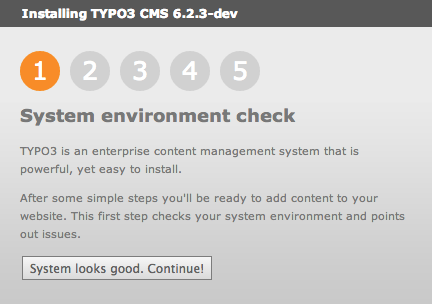
\includegraphics[width=\textwidth]{InstallingTYPO3/DoctrineDBAL/01-SystemEnvironmentCheck.png}
			\caption{Installation TYPO3 CMS - 1. Schritt}
			\label{fig:installTYPO3LegacyStepOne}
		\end{subfigure}%
		~ %add desired spacing between images, e. g. ~, \quad, \qquad, \hfill etc.
	%(or a blank line to force the subfigure onto a new line)
		\begin{subfigure}[b]{0.5\textwidth}
			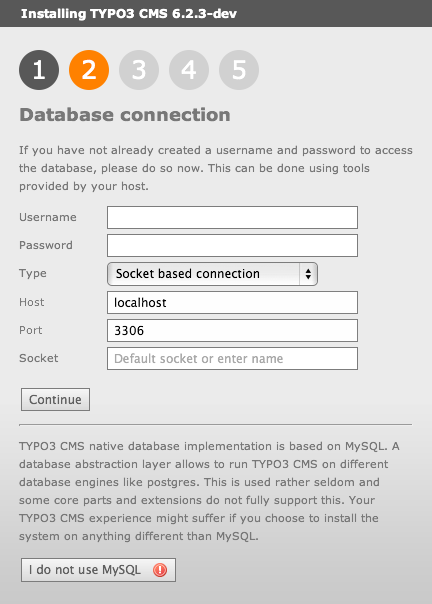
\includegraphics[width=\textwidth]{InstallingTYPO3/Legacy/02-DatabaseConnectionLegacy.png}
			\caption{Installation TYPO3 CMS - 2. Schritt}
			\label{fig:installTYPO3LegacyStepTwo}
		\end{subfigure}
		~ %add desired spacing between images, e. g. ~, \quad, \qquad, \hfill etc.
	%(or a blank line to force the subfigure onto a new line)
		\begin{subfigure}[b]{0.5\textwidth}
			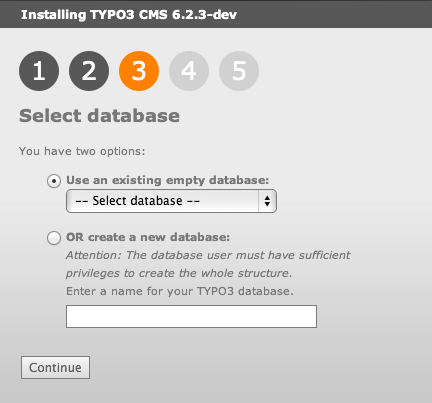
\includegraphics[width=\textwidth]{InstallingTYPO3/Legacy/03-SelectDatabaseLegacy.png}
			\caption{Installation TYPO3 CMS - 3. Schritt}
			\label{fig:installTYPO3LegacyStepThree}
		\end{subfigure}%
		~ %add desired spacing between images, e. g. ~, \quad, \qquad, \hfill etc.
	%(or a blank line to force the subfigure onto a new line)
		\begin{subfigure}[b]{0.5\textwidth}
			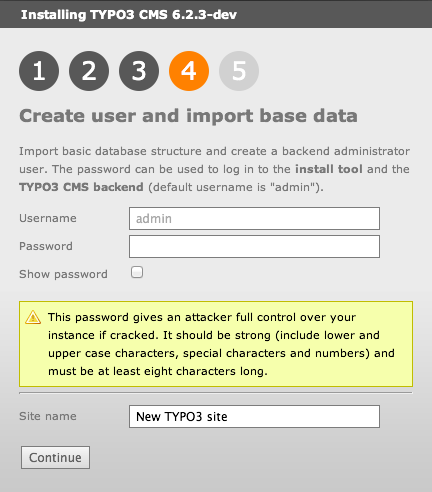
\includegraphics[width=\textwidth]{InstallingTYPO3/Legacy/04-CreateUserAndImportBaseDataLegacy.png}
			\caption{Installation TYPO3 CMS - 4. Schritt}
			\label{fig:installTYPO3LegacyStepFour}
		\end{subfigure}
		~ %add desired spacing between images, e. g. ~, \quad, \qquad, \hfill etc.
	%(or a blank line to force the subfigure onto a new line)
		\begin{subfigure}[b]{0.5\textwidth}
			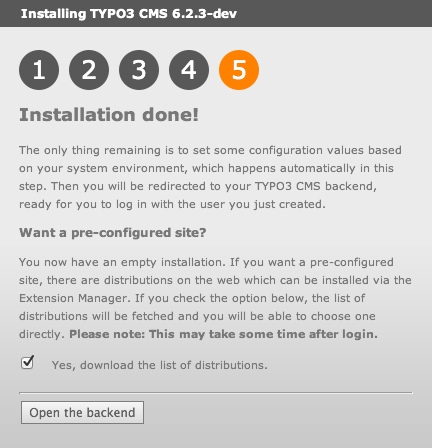
\includegraphics[width=\textwidth]{InstallingTYPO3/Legacy/05-InstallationDoneLegacy.png}
			\caption{Installation TYPO3 CMS - 5. Schritt}
			\label{fig:installTYPO3LegacyStepFive}
		\end{subfigure}%
		\caption{Installation von TYPO3 CMS}
		\label{fig:installationOfTYPO3}
	\end{figure}
